\documentclass[11pt]{article}
\usepackage{amsmath,amssymb}
\usepackage{tikz}
\newdimen\measHT
\newdimen\measDP
\makeatletter
\newcommand\report[3]{%
  \setbox0\hbox{#3}%
  \measHT=\ht0 \measDP=\dp0 %
  \pgfextracty{\dimen6}{\pgfpointdiff{\pgfpointanchor{#1}{center}}{\pgfpointanchor{#1}{north}}}%
  \pgfextracty{\dimen8}{\pgfpointdiff{\pgfpointanchor{#1}{south}}{\pgfpointanchor{#1}{center}}}%
  \typeout{GOT #2 HT=\the\measHT DP=\the\measDP N=\the\dimen6 S=\the\dimen8}}
\makeatother
\begin{document}

\begin{tikzpicture}
  \node[inner sep=0pt] (n0) at (0,0) {T};
  \report{n0}{0}{T}
\end{tikzpicture}
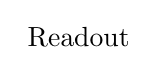
\begin{tikzpicture}
  \node[inner sep=0pt] (n1) at (0,0) {Readout};
  \report{n1}{1}{Readout}
\end{tikzpicture}
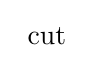
\begin{tikzpicture}
  \node[inner sep=0pt] (n2) at (0,0) {cut};
  \report{n2}{2}{cut}
\end{tikzpicture}
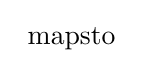
\begin{tikzpicture}
  \node[inner sep=0pt] (n3) at (0,0) {mapsto};
  \report{n3}{3}{mapsto}
\end{tikzpicture}

\begin{tikzpicture}
  \node[inner sep=0pt] (n4) at (0,0) {Reset};
  \report{n4}{4}{Reset}
\end{tikzpicture}
\begin{tikzpicture}
  \node[inner sep=0pt] (n5) at (0,0) {x};
  \report{n5}{5}{x}
\end{tikzpicture}
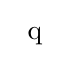
\begin{tikzpicture}
  \node[inner sep=0pt] (n6) at (0,0) {q};
  \report{n6}{6}{q}
\end{tikzpicture}
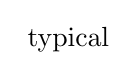
\begin{tikzpicture}
  \node[inner sep=0pt] (n7) at (0,0) {typical};
  \report{n7}{7}{typical}
\end{tikzpicture}
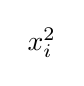
\begin{tikzpicture}
  \node[inner sep=0pt] (n8) at (0,0) {$x_i^2$};
  \report{n8}{8}{$x_i^2$}
\end{tikzpicture}
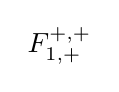
\begin{tikzpicture}
  \node[inner sep=0pt] (n9) at (0,0) {$F_{1,+}^{+,+}$};
  \report{n9}{9}{$F_{1,+}^{+,+}$}
\end{tikzpicture}
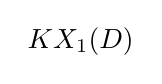
\begin{tikzpicture}
  \node[inner sep=0pt] (n10) at (0,0) {$KX_1(D)$};
  \report{n10}{10}{$KX_1(D)$}
\end{tikzpicture}
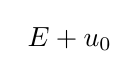
\begin{tikzpicture}
  \node[inner sep=0pt] (n11) at (0,0) {$E+u_0$};
  \report{n11}{11}{$E+u_0$}
\end{tikzpicture}
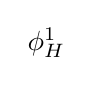
\begin{tikzpicture}
  \node[inner sep=0pt] (n12) at (0,0) {$\phi_H^1$};
  \report{n12}{12}{$\phi_H^1$}
\end{tikzpicture}
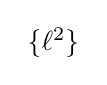
\begin{tikzpicture}
  \node[inner sep=0pt] (n13) at (0,0) {$\{\ell^2\}$};
  \report{n13}{13}{$\{\ell^2\}$}
\end{tikzpicture}
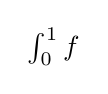
\begin{tikzpicture}
  \node[inner sep=0pt] (n14) at (0,0) {$\int_0^1 f$};
  \report{n14}{14}{$\int_0^1 f$}
\end{tikzpicture}
\begin{tikzpicture}
  \node[inner sep=0pt] (n15) at (0,0) {$\frac{1}{2}$};
  \report{n15}{15}{$\frac{1}{2}$}
\end{tikzpicture}
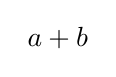
\begin{tikzpicture}
  \node[inner sep=0pt] (n16) at (0,0) {$a+b$};
  \report{n16}{16}{$a+b$}
\end{tikzpicture}
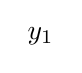
\begin{tikzpicture}
  \node[inner sep=0pt] (n17) at (0,0) {$y_1$};
  \report{n17}{17}{$y_1$}
\end{tikzpicture}
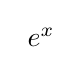
\begin{tikzpicture}
  \node[inner sep=0pt] (n18) at (0,0) {$e^x$};
  \report{n18}{18}{$e^x$}
\end{tikzpicture}
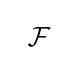
\begin{tikzpicture}
  \node[inner sep=0pt] (n19) at (0,0) {$\mathcal{F}$};
  \report{n19}{19}{$\mathcal{F}$}
\end{tikzpicture}
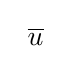
\begin{tikzpicture}
  \node[inner sep=0pt] (n20) at (0,0) {$\overline{u}$};
  \report{n20}{20}{$\overline{u}$}
\end{tikzpicture}
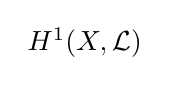
\begin{tikzpicture}
  \node[inner sep=0pt] (n21) at (0,0) {$H^1(X,\mathcal{L})$};
  \report{n21}{21}{$H^1(X,\mathcal{L})$}
\end{tikzpicture}
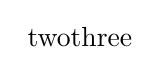
\begin{tikzpicture}
  \node[inner sep=0pt] (n22) at (0,0) {two\\three};
  \report{n22}{22}{two\\three}
\end{tikzpicture}
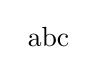
\begin{tikzpicture}
  \node[inner sep=0pt] (n23) at (0,0) {a\\b\\c};
  \report{n23}{23}{a\\b\\c}
\end{tikzpicture}
\end{document}
